\chapter{Design and Implementation}

\section{Architectural overview}

\begin{figure}[H]
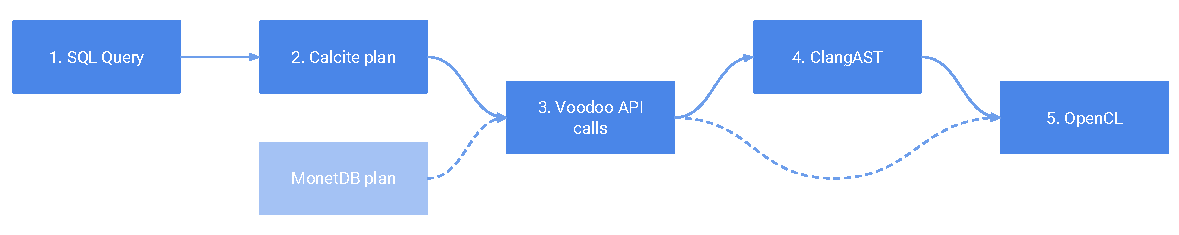
\includegraphics[width=\linewidth]{design-and-implementation/representations.pdf}
\centering
\caption{Translation process from an SQL query to OpenCL code}
\label{fig:translation-process}
\end{figure}

Figure \ref{fig:translation-process} shows our overall approach to processing a query. Starting with an SQL query, we first generate a logical plan, consisting of relational algebra expressions. These relational algebra expressions are then translated to Voodoo vector algebra. An abstract syntax tree is built up from the Voodoo vector algebra, and this AST is then used to generate OpenCL code, which we then run to produce a final result. Appendix \ref{appendix:full-query} shows an example of a query going through this full process.

The dashed lines in figure \ref{fig:translation-process} show the existing approach, preceding our work. This included a comprehensive plan compiler, able to process MonetDB plans, and an implementation of Voodoo, which translated Voodoo vector expressions directly to OpenCL code, using string streams. As shown, our approach represents an almost entirely new implementation. The benefit of this is that we are able to provide an interactive SQL front-end and a more versatile approach to code generation.

We use various frameworks and technologies to implement our approach, some of which are described in section \ref{section:tech}. Figure \ref{fig:voodoo-architecture} provides an overview of the full architecture. Elements in purple represent parts of the architecture which we have implemented, whilst blue elements represent components of the frameworks, libraries, or existing code which we heavily use.

In brief, translation from an SQL query to Voodoo API calls is done in Java, by building on top of the Apache Calcite framework. This involves implementing an adapter to handle data access and processing, which we describe in detail in section \ref{section:sql-to-voodoo}. Translation from Voodoo to OpenCL is done in C++, and makes use of Clang. Here, we have developed from scratch an implementation of the Voodoo API, which we discuss in section \ref{section:voodoo-to-opencl}.

\begin{figure}[p]
\vspace*{-1.4cm}
\makebox[\linewidth]{
    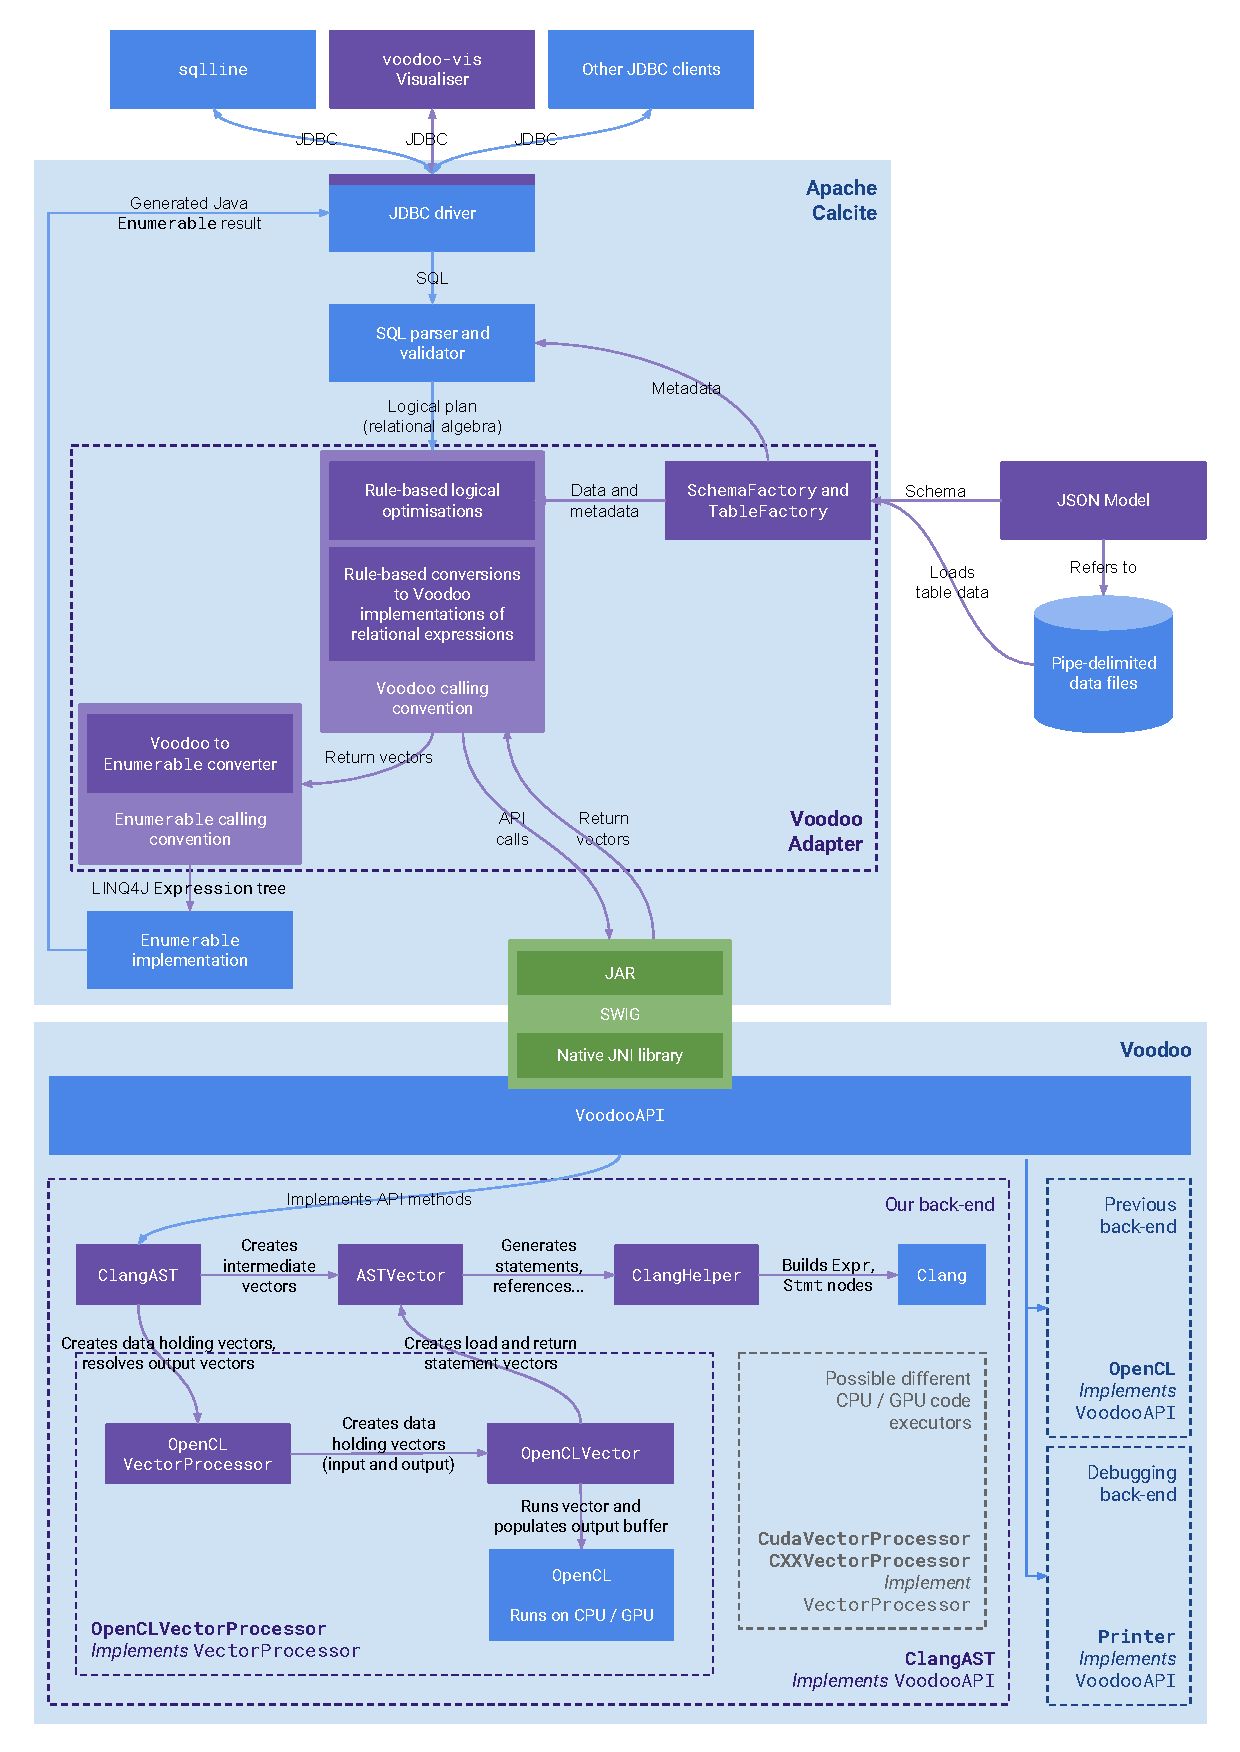
\includegraphics[width=1.1\linewidth]{design-and-implementation/project-architecture.pdf}
}
\centering
\vspace*{-0.7cm}
\caption{An architectural overview of our Voodoo-based query processor}
\label{fig:voodoo-architecture}
\end{figure}

\section{Technical background}
\label{section:tech}

\subsection{Voodoo}\label{original-voodoo-impl}

As we discussed in the introduction, \emph{Voodoo} \cite{Pirk:2016:VVA:3007328.3007336} is a vector algebra which can be used as an intermediate representation between a database query and generated code for that query. It consists of functions defining vector operations, such as the binary operations \texttt{Add} or \texttt{BitwiseAnd}, and more complex or specific operations such as \texttt{Gather}, \texttt{Zip} and \texttt{FoldMin} (which are explained in detail in appendix \ref{appendix:api}). A sequential aggregation query is shown below in figure \ref{fig:short-query}, which sums the balance of all the bank accounts with more than £10,000 on them. The corresponding (simplified) Voodoo program would load the column of the table in memory, filter the column according to the fixed predicate and then aggregate it. We recommend reading the appendix \ref{appendix:full-query} for a deeper understanding.

\begin{figure}[h]
    \centering
\begin{subfigure}[h]{0.39\textwidth}
    \centering
\begin{lstlisting}[language=SQL]
SELECT SUM("account_balance")
FROM account
WHERE account_balance > 10000
\end{lstlisting}
    %\caption{Evaluating \ref{fig:simple-query} using bulk processing}
    \label{fig:short-query-sql}
\end{subfigure}
\begin{subfigure}[h]{0.59\textwidth}
    \centering
\begin{lstlisting}
balance = Load("account_balance")
big_balances = Greater(balance, 10000)
aggregated_balances = FoldSelect(big_balances)
result = FoldSum(aggregated_balances)
\end{lstlisting}
    \label{fig:short-query-vdl}
\end{subfigure}
    \caption{An intuition on Voodoo (ignoring keypaths, some vectors not shown)}
    \label{fig:short-query}
\end{figure}

The existing Voodoo implementation (which we will often refer to as the \emph{back-end}) included a high-performance database \emph{kernel}\footnote{We use kernel to refer to the query processing engine at the core of the database, here the part that evaluates Voodoo expressions.} written in C++ that implemented the \texttt{VoodooAPI} (an interface of the different vector functions in Voodoo). This implementation is called the original \texttt{OpenCL} back-end as opposed to the new \texttt{ClangAST} back-end (which also generates OpenCL). The former can generate highly performant the OpenCL code for the TPC-H queries\footnote{The TPC-H Benchmark is an industry-standard benchmark for comparing the OLAP performance of database systems. It consists of a set of complex queries that run on a specific single databases schema. The full specification is available at \url{http://www.tpc.org/TPC_Documents_Current_Versions/pdf/tpc-h_v2.17.3.pdf}.}, whose Voodoo representations (the \texttt{VoodooAPI} calls) were derived from a MonetDB plan (see figure \ref{fig:translation-process}). The data was loaded from a MonetDB datafarm that was set up separately and loaded in memory before running the queries. There was also another implementation of the \texttt{VoodooAPI}, called the \texttt{Printer}, that proved useful when debugging the front-end. This implementation prints the Voodoo programs as the Voodoo functions were called instead of actually evaluating anything. Figure \ref{fig:voodoo-architecture} shows how the \texttt{VoodooAPI} and existing implementations fit into our overall architecture.

\subsection{Apache Calcite}

\emph{Apache Calcite} \cite{Begoli:2018:ACF:3183713.3190662} is a software framework that provides query language support, query optimisation and query processing, and is used by several popular data processing systems, particularly those in the Hadoop ecosystem. We use it mainly to translate SQL queries to a Voodoo implementation (described in section \ref{section:sql-to-voodoo}).

Whilst Calcite is written entirely in Java, which ocassionally makes interaction with the Voodoo kernel difficult, Calcite was chosen as the framework on which to develop our front-end, for the following reasons:

\begin{enumerate}
    \item Calcite is fairly widely adopted, and with this comes open-source friendliness and stability. In our use of Apache Calcite during this project, we have only encountered two critical unresolved bugs.
    \item By building on top of Calcite, we benefit from not having to entirely implement SQL parsing and validation, JDBC compliancy, and default operator implementations (which are useful when the Voodoo implementation of an operator would be beyond the scope of this project) ourselves.
\end{enumerate}
 
From this point, we assume a comprehensive understanding of the Apache Calcite framework, which is described in detail in appendix \ref{appendix:calcite}.

\subsection{SWIG\label{swig}}

The Simplified Wrapper and Interface Generator (\emph{SWIG}) \cite{Beazley:1996:SEU:1267498.1267513} allows the call to native C++ function in various languages and in particular Java. It requires to write an interface file containing the list of existing C++ classes, types, and methods we want to expose to Java that SWIG will then compile.

In our case, SWIG generates both a \emph{Java Native Interface} (JNI) shared library from compiling the exposed C++ code along with a corresponding JAR that contains the matching Java classes, types and methods that we can import as an external library in Calcite. SWIG handles most of the harmonisation between C++ and Java like respecting C++ virtual function calls, class inheritance, handling pointers, memory ownership (the generated Java classes are in fact just wrappers around the C++ pointers to the underlying C++ classes), serialisation of most types, and offers other features described later (see \ref{swig features}).

\subsection{OpenCL}

The Open Computing Language (OpenCL) is a framework that allows for programming on several target platforms, notably CPUs and GPUs based on C99 and more recently C++11, to run parallel computing tasks. There are several reasons OpenCL which make it fit very well in the project. Indeed it is written in C and also provides C++ bindings for both Linux and Darwin\footnote{For now. Apple has recently announced the deprecation of OpenCL and OpenGL on MacOS 10.14...}, both operating systems Voodoo was desired to be able to run on. As discussed below (\ref{clang-ast-noot}) OpenCL is also compatible with the Clang AST library which was able to generate version compatible code that could be compiled by OpenCL immediately. The original implementation also already used OpenCL which made it easy to get started since the library was already integrated in the project. Although OpenCL's biggest rival, CUDA, may be faster \cite{article}, OpenCL was preferred because of greater flexibility which fits well into the portability idea of Voodoo, and is not proprietary.

\subsection{Clang AST}\label{clang-ast-noot}

Clang AST is an abstract syntax tree that is designed to represent C-like languages like C++ but also OpenCL. It is used in the Clang compiler and is designed mainly for internal use. It is not documented well, with its only documentation being the auto generated doxygen\footnote{\url{https://clang.llvm.org/doxygen/}}. Most functions are not documented and have no comments. This made learning how to use the Clang AST very difficult — it required a lot of experimentation. It was especially challenging for the OpenCL types, which are a more recent addition to the Clang AST, and as such are much harder to find information about.

The Clang AST is also not designed for code generation and we were not able to find any examples of it being used for this purpose. After a spike during checkpoint 2 to evaluate the other AST options that existed, it was still chosen to be used for our code generation because it was the only library that offered a complete representation of OpenCL and that could convert the AST into code\footnote{Making our own OpenCL AST for the project might have also worked, however it would have been hard to maintain over time.}. Although sometimes making OpenCL specific symbols appear in the code can be quite challenging, we have always been able to generate OpenCL code that would compile.

To help us overcome the problem of initially learning Clang, we kept a side project for a few weeks, which was an extension of the code written during the spike, which goal was to create an AST for a particular query. This allowed us to learn how to create structs, for loops, if statements, member expressions, binary expressions, OpenCL keywords, and many more. What we learnt from hard coding this query was then used when developing the back-end.

\section{Generating Voodoo from SQL using Apache Calcite}
\label{section:sql-to-voodoo}

Our first significant deliverable is a database front-end, which, for the first time, allows support for arbitrary SQL queries to be processed on arbitrary schemas using a Voodoo implementation. In the absence of a storage manager, we have also written a basic data loader that allows Calcite to query real data.

Our use of Apache Calcite is rather novel. To our knowledge, there is no open-source Apache Calcite adapter that interfaces directly with a database back-end, rather than producing a textual format (such as SQL, Pig Latin or JSON), or using the Java \texttt{Enumerable} convention for query processing. Our approach posed several unique technical challenges, which are discussed in further detail in this section.

\subsection{Defining schemas and importing data}

Apache Calcite works on the assumption that it knows a lot about your data — it provides a data-source adapter interface that developers must implement, providing schema information, data access paths, type information and statistics.

The Voodoo back-end, however, does not have a storage manager, or any kind of catalog for storing metadata such as statistics. Instead, bench-marking was done by first loading data from MonetDB's storage.

Whilst wanting to reduce our dependencies on MonetDB's components, it would be beyond the scope of this project to develop our own storage manager. As such, we decided to encode the schema information and metadata directly into a JSON model that is passed to Apache Calcite. The data itself would be loaded in byte buffers, meaning it could be copied directly into OpenCL memory with no additional processing.

\paragraph{Schemas}

Our \texttt{SchemaFactory} can be used to pass configuration parameters defined in the JSON model to the Voodoo back-end. Currently, it provides the \texttt{implementation} parameter, which allows users to define which implementation of the Voodoo API to use. Other useful configuration options, such as whether OpenCL should run on a GPU or CPU, could also be added here.

\paragraph{Tables}

The bulk of the work is done in our \texttt{TableFactory}, which is how we allow users to define custom tables. Here, the JSON model must provide a table name, and a list of columns, with each of their names and SQL types. Additionally, users can provide details of foreign keys, which can be used to produce a simpler and more efficient Voodoo representation for some queries, in particular those with joins.

We register a table of that name and type in our adapter, allowing for SQL queries to be validated. The type is converted to a \texttt{VoodooType}, which we use to translate between SQL, Java and C++ types. We also store this in our \texttt{Table} implementation, as it is useful when evaluating row-expressions, and returning a final result.

\begin{table}
    \centering
    \begin{tabularx}{\linewidth}{l l L L L H}
        \hline
        SQL type & \texttt{VoodooType} & Java type (\texttt{Voodoo} convention) & Java type (\texttt{Enumerable} convention) & C++ type (Voodoo kernel) & Voodoo representation \\
        \hline
        \texttt{BOOLEAN} & \texttt{VBOOLEAN} & \texttt{Boolean} & \texttt{Boolean} & \texttt{int} (or \texttt{char}) & valued 0 or 1 \\
        \texttt{CHAR} & \texttt{VCHAR} & \texttt{Character} & \texttt{String} & \texttt{int} (or \texttt{char}) & valued between 0 and 255 \\
        \texttt{INT} & \texttt{VINTEGER} & \texttt{Integer} & \texttt{Integer} & \texttt{int} (or \texttt{long}) &  \\
        \texttt{BIGINT} & \texttt{VBIGINT} & \texttt{Long} & \texttt{BigInteger} & \texttt{int} (or \texttt{long}) &  \\
        \texttt{DECIMAL(p, s)} & \texttt{VDECIMAL} & \texttt{Double} & \texttt{BigDecimal} & \texttt{int} (or \texttt{long} or \texttt{double}) & scaled by $10^\texttt{s}$ \\
        \texttt{DATE} & \texttt{VDATE} & \texttt{Integer} & \texttt{Calendar} & \texttt{int} & days since epoch \\
        \texttt{CHAR(n)} & \texttt{VSTRING} & \texttt{String} & \texttt{String} & \texttt{int} & dictionary-encoded \\
        \texttt{VARCHAR(n)} & \texttt{VSTRING} & \texttt{String} & \texttt{String} & \texttt{int} & dictionary-encoded \\
        \hline
    \end{tabularx}
    \caption{Representation of supported data-types}
    \label{tab:types}
\end{table}

The data for each column is stored in a byte buffer. Originally, we would populate these buffers with random data, based on the column's type. However, in order to improve testability and usability, we later decided to write a simple data loader. In our model JSON, a \texttt{dataSource} property is provided for each table, stating the path, relative to the model, of a pipe-delimited data file, used to populate the table. We read the data file, and write the data to byte buffers for each column, using the representation defined in table \ref{tab:types}. Noteably, as strings are not supported by our back-end, they are stored in a schema-wide dictionary and the integer value is placed in the byte buffer.

Whilst loading the data, we can calculate statistics that can be used by planning rules to reach a better logical plan. Currently, we just provide the cardinality of the table, although it should be relatively straight-forward to extend this to a histogram, which would allow us to provide stronger guarantees to the back-end and hence produce more efficient code without sacrificing correctness.

Finally, we create an \texttt{ASTVector} for each column, which we store for access by relational expression implementations on the table. We additionally keep a reference to the byte buffers, to keep them from going out of scope and thus being freed by Java's garbage collector.

\subsection{Translating relational operators to Voodoo}

Apache Calcite provides an SQL parser and validator, and as such we start with a tree of logical relational operations (similar to those depicted in figure \ref{fig:improving-qpt}). We translate this tree to Voodoo algebra in three stages:
\begin{enumerate}
    \item \emph{We optimise the logical plan}, using hundreds of planner rules. Most of these are provided by Calcite, and make various useful optimisations to avoid excessive work (such as pushing filters and projects into joins). Some are written for Voodoo in particular, such to push projects into table scans (since our Voodoo back-end reads data as columns).
    \item \emph{We assign each operation a calling convention trait}, which chooses the data processing system used to implement that operation. What this means is that a query could potentially access several heterogeneous data sources (\texttt{Cassandra}, \texttt{Spark}, \texttt{MongoDB} and \texttt{Hive}, for example, all have their own calling conventions). However, in our case, either the \texttt{Voodoo} or \texttt{Enumerable} calling convention will be assigned. Operators with a \texttt{Voodoo} calling convention will be implemented by our Voodoo back-end, whilst \texttt{Enumerable} operators build up a tree of LINQ4J \texttt{Expressions}. Additional converter nodes are inserted between different calling conventions.
    \item \emph{We implement each node in the plan}. Once the plan has been optimised, calling conventions assigned, and converters added where necessary, the plan is implemented, starting at the root node. This happens as follows:
    \begin{enumerate}
        \item Subtrees of \texttt{Enumerable} operators build a tree of expressions that implement their operations. This is used to generate the source code for a Java class with a \texttt{bind()} method, which returns an enumerable object containing the result.
        \item Converter nodes get the result of their input subtree and provide it in a format which is useable by the calling convention that follows.
        \item Subtrees of \texttt{Voodoo} operators are implemented by performing a depth-first post-order traversal of the tree. Each relational expression implementation overrides a \texttt{getColumns()} method and an \texttt{implement()} method. \texttt{getColumns()} returns the columns that result from the evaluation of the relational expression, whilst \texttt{implement()} populates these columns. In \texttt{implement()}, we first recursively implement any children nodes. Then, we can access the columns produced by the child, and use calls to the Voodoo API to apply our own vector operations, in order to implement the relational expression represented by our current node.\footnote{This step can range from being relatively simple to rather involved. A full description of how we handle each type of relational expression is provided in appendix \ref{appendix:rel}.} Finally, we make the resulting columns accessible to our parent node.
    \end{enumerate}
\end{enumerate}

The first two stages are done by the \texttt{VolcanoPlanner} planner engine. This uses a dynamic programming algorithm to fire planner rules until the estimated cost of the plan levels off. Such an approach has several limitations:
\begin{enumerate}
    \item Rule-based logical optimisation is fragile to begin with. When this is combined with questionable or non-existent cost models in existing adapters, it becomes quite difficult to make the planner engine apply our rules. Furthermore, Calcite provides hundreds of rules by default, and disabling them is both tricky and can have unintended side-effects. As such the planning process is incredibly difficult to debug.
    \item We use Calcite's default configuration for the planner engine, which means that it is both \texttt{patient} and \texttt{ambitious}. As a result Calcite applies rules exhaustively. This can be extremely slow — it takes over 15 seconds to plan some TPC-H queries which have several joins! This likely could be resolved by changing the configuration or the supplied rules. However, since we are not concerned with the efficiency of the front-end, this remains an open issue.
    \item There is a known, unresolved issue (\hyperlink{https://jira.apache.org/jira/browse/CALCITE-2015}{CALCITE-2015}), in which Calcite's planner can get stuck in a cycle, generating an infinite number of plans. When it eventually gives up, it can return an incompatible plan. We have to manually handle this case in each of our rules.
\end{enumerate}

Each of our \texttt{Voodoo} operators are associated with low costs, in an attempt to get the planner to use them where possible. Furthermore, in order to generate viable plans, we developed three conditions which should, in general, hold for every planner rule which converts logical operators into their \texttt{Voodoo} equivalent. Concretely, the node to be replaced:
\begin{enumerate}
    \item Must be a logical version of the operator with which is is to be replaced.
    \item Must only have children that also use the \texttt{Voodoo} calling convention.
    \item Must not include a row expression which we cannot currently implement (see subsection \ref{sub:rex}).
\end{enumerate}

Currently, we provide \texttt{Voodoo} conversion rules and implementations for the \texttt{TableScan}, \texttt{Project}, \texttt{Filter}, \texttt{Join} and \texttt{Aggregate} operators. In appendix \ref{appendix:rel}, we describe in detail how each of these operators is converted into Voodoo.

For the relational operators for which we do not currently provide implementations (such as \texttt{Sort}, which is discussed in subsection \ref{sub:top-n}), we provide a converter that translates a Voodoo result to the \texttt{Enumerable} convention. Calcite's JDBC driver also relies upon this converter.

It works by first calling \texttt{returnVector} on the result vectors. We allocate a byte buffers of the correct size in Calcite, and copy the data from the result vectors. Once we have the data, we iterate through the columns and build up lists of Java expressions representing the literal values in each row. We finally apply a wrapper which converts our array into an \texttt{Enumerable} class, and pass the result to an \texttt{EnumerableRelImplementor}, which can append on any remaining processing before returning the final result set.

It is important to note that there are two major limitations of this approach:
\begin{enumerate}
    \item The \texttt{Enumerable} convention is quite inefficient, both in terms of speed and memory usage. Relying on it to do any significant amount of data processing is a bad idea in general.
    \item There is a strict 64KB byte-code size limit on Java methods, and the \texttt{Enumerable} implementation works by generating Java source code. Since we pass in our data directly as literal expressions (rather than through a file, for example), should the size of the result approach 64KB, the \texttt{Enumerable} implementation will fail to compile its source code, and no result will be returned.
\end{enumerate}
These issues could be resolved by implementing more functionality in the \texttt{Voodoo} convention, and by either rewriting the converter to save results to a \texttt{Scannable} file format, or by implementing parts of the JDBC driver ourselves.

\subsection{Translating row expressions to Voodoo}
\label{sub:rex}

\begin{figure}
    \centering
    \begin{tabular}{|c|}
    \hline
    \begin{lstlisting}[language=SQL]
"l_shipmode" = 'MAIL'
AND "l_shipdate"
  BETWEEN date '1996-01-01'
  AND date '1996-01-01' + interval '1' year
    \end{lstlisting} \\
    \hline
    \end{tabular}
    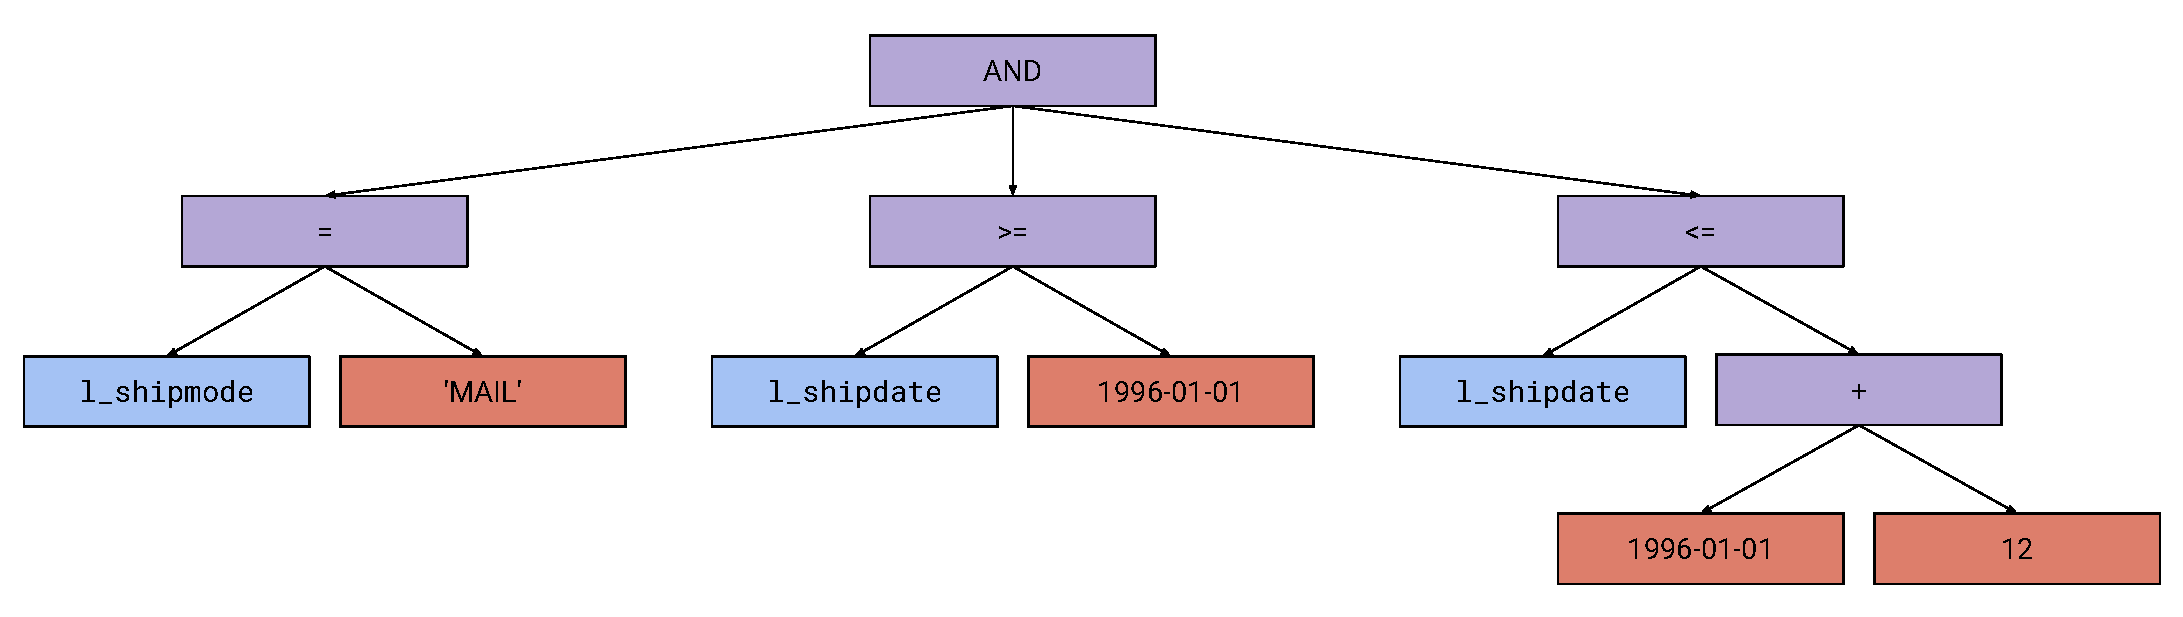
\includegraphics[width=\linewidth]{design-and-implementation/rex-node.pdf}
    \caption{An SQL row expression and the tree of \texttt{RexNode}s which represent it}
    \label{fig:rex}
\end{figure}

A row expression is an expression to be evaluated over a single tuple. Figure \ref{fig:rex} shows an example. We represent row expressions in the front-end as a tree of \texttt{RexNode}s. We support three implementations of \texttt{RexNode}: operator calls (shown in purple), input column references (shown in blue) and literal values (shown in red).

We have developed a \texttt{VoodooRexImplementor}, which uses a visitor pattern to implement \texttt{RexNode} trees in Voodoo vector algebra. Unlike the implementation for relational expressions, which makes API calls while traversing the tree, here we use a command pattern to build an ordered list of API calls, which are called once the entire row expression has been traversed. This gives us greater control as we can modify previous calls.

\paragraph{Literal values}
We first attempt a translation from Calcite's representation to Voodoo's representation, as described in table \ref{tab:types}. This is based on the literal's SQL type. However, this is sometimes insufficient to actually determine the representation (since this depends on the column's type, rather than the literal's).

\paragraph{Input references}
Input references are resolved by reading the columns of any children of the current relational operator, which must be passed to the row-expression implementer by the relational operator node. We also store a reference to the Voodoo type of the input column.

\paragraph{Operator calls}
We iterate through the operator call's children, implementing each of them. This will return a list of commands, together with type information. We ensure that the types are compatible, and make adjustments to the representation of literals where necessary. At this point, we add the expression(s) required to implement the operator. This is almost always very straight-forward: we currently support: $+$, $-$, $\times$, $/$, $\%$, $=$, $\not=$, $<$, $>$, $\leq$, $\geq$, $\land$ and $\lor$, which can all be implemented in at most three Voodoo vector expressions.

\paragraph{Other row expressions}
Whilst we are able to implement most common SQL row expressions, there are some types that we do not support. Notably, this includes the \texttt{CASE} statement, as well as any operations on string types except for equality checks (this is a drawback of our dictionary-based representation method for strings). We provide a \texttt{VoodooRexChecker} that checks whether or not a row expression is able to be implemented. Our planner rules apply this check, and if it does not pass, we will instead use the \texttt{Enumerable} convention to get a result.

\subsection{Communicating with the Voodoo Kernel}\label{swig features}

We use SWIG (\ref{swig}) to expose the \emph{Voodoo API} and the different implementations we want to call from Calcite (i.e. the \texttt{Printer}, the original \texttt{OpenCL} and our new \texttt{ClangAst} back-end). SWIG is very well suited in this case since Voodoo is a vector algebra language that contains only a limited set of functions (\texttt{Range, Add, etc.}) that were implemented in C++; functions that can each be exposed to Calcite to run the corresponding Voodoo algebra. Furthermore, this design means that the back-end can be modified more freely since the interface acts as an explicit encapsulation layer which decouples it from the front-end.

Therefore, the SWIG interface file consists of the different Voodoo functions along with their arguments. Those arguments are mostly the following important classes along with sometimes some primitive types:

\begin{enumerate}
    \item The abstract class \texttt{StructuredVector} which represents the columns of the table we are processing. The real type of those depend on which back-end we are using. Each back-end being required to extend the class to make use of its own kind of vectors to hold specific metadata for this back-end. In our case and as can be seen on the architecture diagram (\ref{fig:voodoo-architecture}) we extended it to an \texttt{ASTVector} which notably represents type of statement it will be in the AST along with its arguments. In the code snippet below (Fig \ref{fig:java-voodoo-api}) the \texttt{vTimesTwo} vector will hold a Clang binary statement adding the two arguments; arguments being \texttt{v} in this case.
    
    \item A keypath defines a property of the object it refers to (e.g. \texttt{object.key.subkey} where \texttt{.key.subkey} is the keypath). Vectors in Voodoo can have multiple columns to express the idea of \emph{control vectors}. More concretely, vectors with multiple keypaths correspond to an array of \texttt{struct} in OpenCL. A \texttt{KeyPath} class is used to describe those.
\end{enumerate}

\begin{figure}[h]
    \centering
\begin{lstlisting}[frame=single, language=Java]  
VoodooAPI api = Voodoo.getVoodooImplementation(Printer);
StructuredVector v = api.Load(/* column */); // Loads a stored column of a table
StructuredVector vTimesTwo = api.Add(v, v);  // vTimesTwo = 2 * v
\end{lstlisting}
    \caption{Simplified example of how to write Voodoo in Java, omitting \texttt{KeyPath} for brevity}
    \label{fig:java-voodoo-api}
\end{figure}

A SWIG interface file already existed containing the classes described above when we started on the project because of previous research on Voodoo with a Scala project dating from a couple of years ago. After fixing the bugs that appeared while the development was idle, getting started with SWIG was very straight forward, it was down to implementing a new back-end by extending the \texttt{VoodooAPI} and \texttt{StructuredVector} class and then exposing those in the SWIG interface file. Proceeding like so had the advantage that we were not breaking backwards compatibility and we would also be able to use in the front-end some other back-ends. We could rely on various existing features already implemented and avoided multipling the number of SWIG interfaces file.

However, we did not rush into this decision, and we implemented a spike during Checkpoint 1 to try and come up with and alternative SWIG API. There are indeed a significant trade-offs in using this design. Extending the \texttt{VoodooAPI} creates a great deal of coupling, and means our back-end would notably use the \texttt{StructuredVector} and \texttt{KeyPath class} classes; classes for which the design would make it quite a lot harder to work with than to just create our own. We would not use most of their features and they were hard to elegantly extend. This choice would also significantly influence the design of both the front-end and back-end, and would mean that we sometimes had to find ad-hoc workarounds. Eventually it was decided to go with the option of extending the API, because we wanted to use the \texttt{Printer} implementation, at the cost of a design with a higher level of coupling.

Integration tests ensure there is always high quality level of communication between the front-end and back-end. These tests included, at first, only the \texttt{Printer} implementation since it was used extensively by the front-end for debugging. Later, they were extended to the \texttt{ClangAst} back-end when its development started. Writing good integration tests is hard, especially when interfacing between different languages. SWIG for example helped with a handy type conversion between \texttt{ByteBuffer} in Java and giving a raw \texttt{(void *)} in C++, supposing Java could tune the endianess of the buffers\footnote{Operations with \texttt{ByteBuffer} are big endian by default, but can be changed to use the native order of the computer which C++ uses.}. Raw storage data managed in Calcite is given to the back-end to import into OpenCL memory in the form of vectors (columns) and after the query evaluation the back-end copies the OpenCL memory into a \texttt{ByteBuffer} for Calcite to read. Passing and copying data around like this can seem quite expensive, however Voodoo aspires to be the fastest database \emph{kernel} in the world, as such the focus of the front-end was to provide an optimal user experience.

\section{Generating OpenCL from Voodoo using Clang AST}
\label{section:voodoo-to-opencl}

The process of generating OpenCL code from Voodoo Code is a fivefold process:
\begin{enumerate}
    \item Translating Voodoo operators to AstVectors and ClangAST nodes
    \item Grouping AstVectors into Blocks
    \item Generating the OpenCL code from the Block State
    \item Running the OpenCL Code
    \item Returning the Result
\end{enumerate}


\subsection{Using Clang AST to generate AST components}

The intention of this side of the project was to replace string based code generation with an AST based system. Multiple options were considered for the code generation AST such as the LibClang, Clang plugins, LibTooling and the Clang AST itself, CPPAst and building our own. We used the Clang AST itself as it provided the best utility for generating and producing code. As the Clang AST does not hold guarantees as to changes in future builds, we lock our LLVM version to 8 which supports all the OpenCL code we need to generate.

\subsection{Translating Voodoo to a Clang AST} \label{voodoo-to-ast}

For each Voodoo operator, the relevant section of the final code is generated as ClangAST nodes. This is stored in \texttt{ASTVector}, as well as a list of previously required \texttt{ASTVectors}. This list forms the basis of a directed acyclic graph of dependencies. For calls to the Voodoo operator \texttt{Load} (which set up the inputs to the graph), the implementation specific \texttt{VectorProcessor} handles loading the data and making the data readable by the query executor. We have implemented an OpenCL \texttt{VectorProcessor} that can execute the query on GPU or CPU using OpenCL.

Once this graph has been fully assembled, calls to \texttt{ReturnVector} or \texttt{ReturnMultiVector} will generate another special data holding vector specified by the \texttt{VectorProcessor}. A traversal of the tree will occur and generation of the full Clang AST necessary to calculate the final output held in this vector will take place. This process involves cutting the graph into different \emph{fragments} which can be run in parallel. This fragment graph is also directed and acyclic and is used to generate the combined AST of the full query. Clang then generates OpenCL code from this AST which is loaded into the OpenCL device along with the columns of data needed for this fragment. The code is then executed while recording performance analytics. Finally the output buffers containing the result are read from OpenCL memory and returned to the front-end to be displayed.

\subsection{\texttt{ASTVector} generation}

Each \texttt{VoodooAPI} function uses \texttt{KeyPath} as an argument to specify the member of the input and output vector relevant to the API call. Since we expect tables to be stored in a \emph{column store}\footnote{A column store stores each column of the table separatly as opposed to a row store which store tuples together.}, input vectors can only have a single member and so the keypath is unused for most API calls and can be ignored. Our back-end mainly uses keypaths when constructing or referencing a \texttt{Zip} call, therefore forming an array from a \texttt{struct}.

A detailed description of each \texttt{VoodooAPI} function, and how we generate OpenCL for them using a Clang AST, is provided in appendix \ref{appendix:api}.

\subsection{Grouping \texttt{AstVector}s into Blocks}
The word \emph{block} will refer to a collection of \emph{statements} that belong in the same scope. Any Voodoo function that will make a new scope is called a fragment generator. The word \emph{block} in the report is referred to as a \emph{fragment} in the source code.

The main purpose of grouping \texttt{AstVector}s together into blocks, is so that when generating OpenCL code, the statements that belong in a certain scope are added to that scope.
This structure easily deals with functions that create a new scope such as \texttt{Cross} which creates a for loop inside a another for loop. The statements that belong with the cross (i.e in the inner for loop) are correctly added to the inner for loop's body and the statements that do not belong with the cross are added to the outer for loops.

The current implementation uses a recursive algorithm to achieve this. 

\begin{enumerate}
    \item Starting from the \texttt{ReturnVector}, recursively call the function on the required vectors until a \texttt{Load} statement is hit.
    \item Once a \texttt{Load} statement is hit, we create a new block, add the \texttt{Load} statement to the block and return.
    \item We then continue to traverse the \texttt{ASTVector} dependency graph using a visit-leave depth first search. We recursively generate the block map from this. Adding any following calls from a load statement into the same block unless a special case is found. 
\end{enumerate}

\subsubsection{Scope Cases}

\paragraph{Load}

Load calls increase the scope by generating a new block with a for loop. If the load call is the right branch of a cross call then this block will be placed inside the left branches block (while visit cycle is ongoing), otherwise it is placed within the parent block (while leave cycle is ongoing). All following calls made using load will be placed in this block.

\paragraph{Cross}

Cross calls increase the scope by generating a new block with a for loop. It will visit the left hand side of the call to generate the outer block, and then the right hand side block is placed inside this block with a new dominating iterator.

\paragraph{FoldSelect}

FoldSelect calls increase the scope by generating a new block which is contained by an if statement. All following calls made using the argument that was foldSelected will be placed in this block.

\paragraph{FoldSum, FoldMin, FoldMax}

These calls are named \emph{reducers}, because they reduce the scope of any future calls. From inside a for loop, these calls generate an output value which can only be accessed once the for loop has terminated and cycled through all the values. All following calls using the value of the reduction will be placed in the current block's parent block.

\paragraph{Return}

These calls are not scope changers, but require information about the current block to be correct. Once they have been placed in the correct block, the size of the vector is determined and saved so the output vector as well as the correct bufferSize to pass to the front end.

\paragraph{Unary}

Unary statements are a special case as it is unclear which block the statement belongs in. If it is operating on a value which has just been immediately reduced by a reducer then it is placed in the parent block (one scope up), which the maximum top level parent scope being the function itself outside of any for loops. 

\paragraph{Binary}

Binary statements operate on two vectors and so require special consideration. 
If both of the inputs have been immediately reduced and exist in the same scope, then it is placed afterwards in the same scope. If they exist in different scopes, then it is placed in the latter of the inputs if they are directly or indirectly dependent on each other, if not dependant then another block is created dependant on both inputs and in the same scope.

If only one has been reduced then it is placed in the scope of the unreduced and the reduced input is added as a dependent to the unreduced block.

If neither of the inputs have been immediately reduced and exist in the same scope, then it is placed afterwards in the same scope. 

\subsubsection{Conditions for Merging two Blocks}
\begin{enumerate}
    \item If both blocks are from the same table.
    \item If both blocks are in the same scope (i.e the same parent block).
    \item If one block is not in the other block's list of dependant blocks.
\end{enumerate}

\subsubsection{Our Algorithm}
Let us take a simple query (figure \ref{fig:simpleQuery}) to analyse. Starting at the \texttt{Return} vector, recursively call the algorithm on it's required vector which in this case is an \texttt{Add} vector. The add vector requires 2 vectors, so recurse on the first required vector (left branch of the figure) and then the second required vector (right branch of the figure). It recurses up the left branch until it hits a \texttt{Load} vector.

The \texttt{Load} vector, creates a new block with block number 1 and the load statement (statement number 1) is added to the block and returns (This corresponds with Step 1 shown in figure \ref{fig:fragConstruction}). The \texttt{Project} and \texttt{FoldSum} vectors (statement number 2 and 3 respectively) are added to block 1. As \texttt{FoldSum} is a reducer, the block is closed and added to it's parent block's list of contained blocks which in this case is the base block. The block for the first required vector of the add vector is created. The same process is repeated for the second required vector of the add vector (this corresponds with steps 4 to 6 of Figure \ref{fig:fragConstruction}). 

As the two blocks are reduced and are in the same scope and are from the same table, they can be merged together into one block. A new block is created with block number 3 and all the statements are added to it (this corresponds with step 7 of figure \ref{fig:fragConstruction}). 

A new block is created with block number 4 and the add vector is added. The \texttt{Add} vector is in a different scope than its required vectors and as it depends on the output of it's required vectors, block 4 depends on block 3 (this corresponds with step 8). 

A new block with block number 5 is created for the \texttt{Return} vector; vector which depends on the result of the add, block 5 depends on block 4 (this corresponds with step 9).

\begin{figure}[h]
\centering
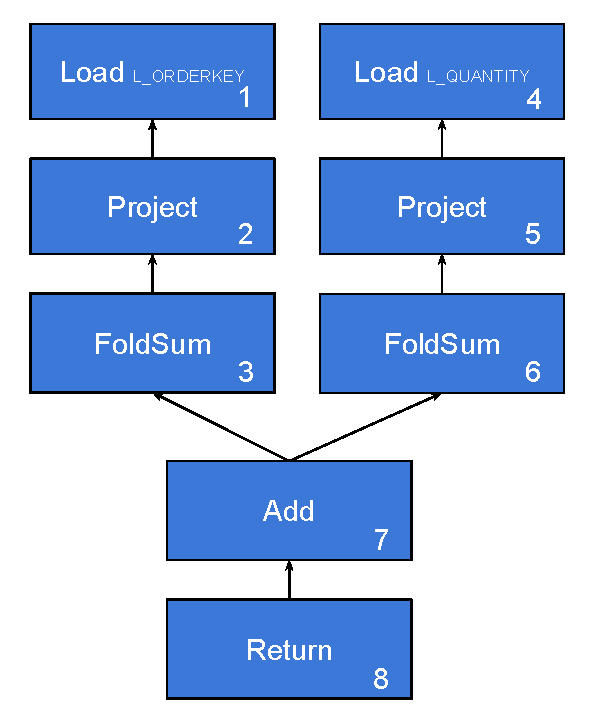
\includegraphics[width=\textwidth,height=5cm,keepaspectratio]{design-and-implementation/SimpleQuery.pdf}
\caption{A simple query which sums all the order keys and all the quantities and add the totals together. (Calls to zip have been removed for brevity)}
\label{fig:simpleQuery}
\end{figure}

\begin{figure}[p]
\centering

\begin{subfigure}{0.99\linewidth}
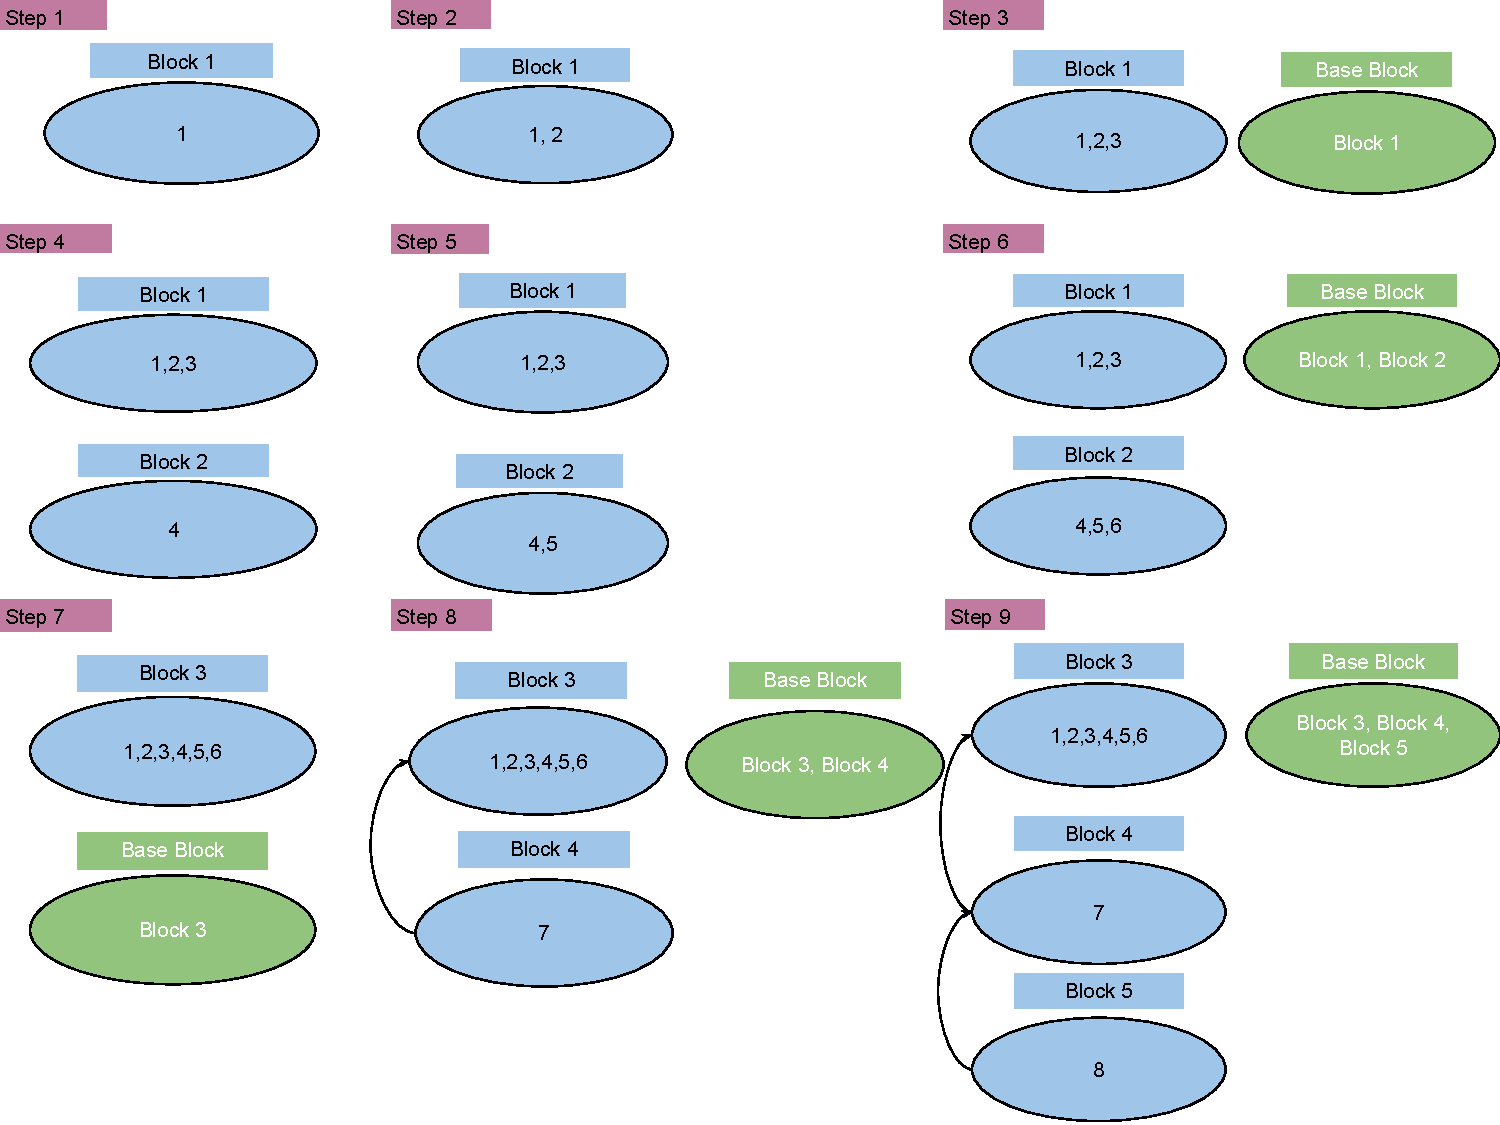
\includegraphics[width=\textwidth]{design-and-implementation/FragmentConstruction.pdf}
\centering
\caption{Block construction for \ref{fig:simpleQuery}}
\label{fig:fragConstruction}
\end{subfigure}
\\[5ex]
\begin{subfigure}{0.7\linewidth}
\begin{lstlisting}[frame=single, language=C]
__kernel void __runFragment0(
    __global int *persitent1,   // L_ORDERKEY column vector
    __global int *persitent5,   // L_QUANTITY column vector
    __global long *persistent10 // Result vector
) {
     int tmp4 = 0;
     int tmp8 = 0;
     for (int dominatingIteratorOffset = 0; 
          dominatingIteratorOffset < 3; 
          dominatingIteratorOffset += 1) {
         int tmp2 = persitent1[dominatingIteratorOffset];
         tmp4 = tmp4 + tmp2;
         int tmp6 = persitent5[dominatingIteratorOffset];
         tmp8 = tmp8 + tmp6;
     }
     int tmp9 = tmp8 + tmp4;
     persistent10[0] = tmp9;
}
\end{lstlisting}
    \caption{OpenCL code for \ref{fig:simpleQuery}}
    \label{fig:opencl-code}
\end{subfigure}

\end{figure}

\subsection{Generating the OpenCL code from the Block State}

Once all the blocks are created, we traverse the blocks that are contained in the base block and for each block, add all the statements that are part of that block to the body of a for loop (unless the block is a foldSelect block in which case, the statements will be added to the body of the if statement) and return. Once all the blocks that are contained in the base block have generated their statements, they are added to the function body and any parameters of the individual blocks are added as function parameters.

The current implementation uses a recursive solution. This algorithm assumes that the statements included in each block are sorted by their statement number. This is enforced by the correct structure of the Voodoo API.

\subsubsection{Our Algorithm}

Let's take the following simple query (Figure \ref{fig:simpleQuery}) as an example again. Once all the blocks have been generated (i.e step 9 of figure \ref{fig:fragConstruction}), we loop through the base block and get the first block that has no dependencies which in this case is block 3.

Block 3 contains 2 \texttt{Load} calls from the same table, which means that block 3 is a for loop block. As block 3 does not contain any blocks, all the statements in block are added to the body of the for loop. and The for loop and any input declarations are returned which are then added to the body of the function. Block 3 is now removed from the list.

Once block 3 is removed, the next block that has no dependencies is retrieved which in this case is block 4. Block 4 is a base level block and so all the statements that belong to it are added immediately to the body of the function. Block 4 is now removed.

Once block 4 is removed, the next block that has no dependencies is retrieved which in this case would be block 5. Block 5 is a base level block and contains only the return statement which is added immediately to the body of the function. Block 5 is now removed.

As there are no more blocks that are contained in the base block, the algorithm is finished and the code generated is ready to be run. The code generated is shown in figure \ref{fig:opencl-code}


\subsection{Running the OpenCL Code}
Loading of data into the OpenCL environment and execution of the code is handled by a \texttt{VectorProcessor}. We have implemented an \texttt{OpenClVectorProcessor} and \texttt{OpenClVector} to allow queries to execute on GPU or CPU using OpenCL.

When resolve is called on a fragment, the code is retrieved and loaded into to the OpenCL environment. Any settings related to OpenCL are also loaded, such as whether to use GPU or CPU. Additionally, for all the parameters used by the code the necessary input buffers containing the input data and empty output buffers are loaded and registered to OpenCL.

Once the input and output has been set up, the code is executed in the OpenCL environment. The time taken is recorded for benchmarking purposes and then the resolved vector is returned to the user, containing pointers to the output buffers, buffer size and type.

\section{Graphical web-interface}

We additionally provide a graphical front-end on top of our Calcite adapter, which displays the Calcite plan, Voodoo vector expressions, OpenCL and result for a query on the TPC-H schema, as shown in figure \ref{fig:q6-vis}.

\subsubsection{Purpose}

Building an interface was not an explicit goal of this project, and as such we did not prioritise its development. However, it does serve a useful purpose, which we claim is threefold:

\begin{enumerate}
\item It shows very clearly the transformations we make to generate OpenCL code from an SQL query, and provides graphical visualisations of the plan at various stages. As such, it is helpful for presenting the work we have done, and explaining how each intermediate representation is reached.
\item It provides a somewhat useful debugging interface. The alternative would be to use Apache Calcite's \texttt{sqlline} command-line interface. However, \texttt{sqlline} has several limitations. Firstly, there is a known issue whereby \texttt{sqlline} truncates long plans. Secondly, viewing the generated Voodoo vector expressions and the generated OpenCL require a different Voodoo implementations (\texttt{Printer} and \texttt{ClangAst} respectively), and hence different JDBC connections, which can be a little tedious to set up. The interface we have built does not require any such setup, and allows us to easily identify where a buggy query has gone wrong.
\item It proves that our database is JDBC-compliant, and provides sample Java code that includes connection configuration. It also demonstrates that we can handle arbitrary SQL queries.
\end{enumerate}

\subsubsection{Implementation}

\begin{figure}[H]
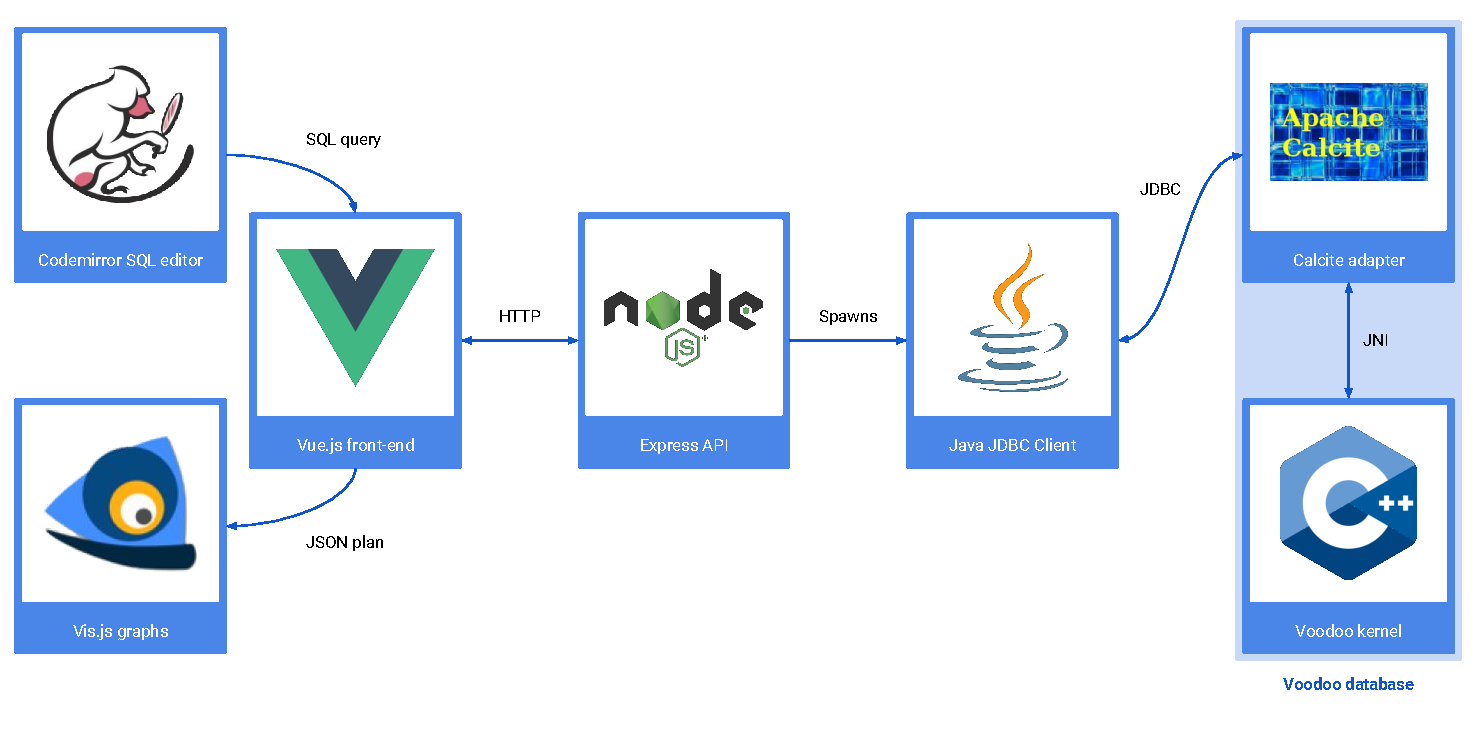
\includegraphics[width=\textwidth]{design-and-implementation/web-interface.pdf}
\centering
\caption{Architecture of the graphical web-interface}
\label{fig:web-interface}
\end{figure}

Figure \ref{fig:web-interface} shows the main components of the web-interface. Since this interface is not considered to be a real deliverable of this project, we favoured design decisions that allowed the most rapid development. As such we have:

\begin{enumerate}
\item A \emph{JDBC client}, written in Java, that connects to our Voodoo implementation via the Calcite adapter. Note that the client never interacts directly with the Voodoo kernel, and so we rely on the kernel outputting Voodoo and OpenCL code, in addition to returning a result via the Calcite adapter. This approach provides a much cleaner interface than using an existing client, say \texttt{sqlline}, and avoids using unmaintained Node.js JDBC libraries.
\item An \emph{Express API}, which accepts HTTP \texttt{GET} requests for a query. It returns a JSON, built from the output of the JDBC client, containing the plan, Voodoo, OpenCL and result for a query as well as any warnings or errors reported. This approach was much faster than using one of Java's more verbose HTTP server frameworks.
\item A \emph{Vue.JS front-end}, which uses CodeMirror to provide an editor with SQL syntax highlighting and autocompletion. Queries are sent to the API, and we parse the response, using a hierarchical depth-first search starting from the returned vector, to build up the list of nodes and edges in a connected graph of the plan. The distances from the returned vector are used to define the $y$-coordinates ("levels") of operator nodes in the final graph, and vis.js then calculates $x$-coordinates using a physics simulation with spring forces between nodes.
\end{enumerate}

\begin{figure}[b!]
    \centering
    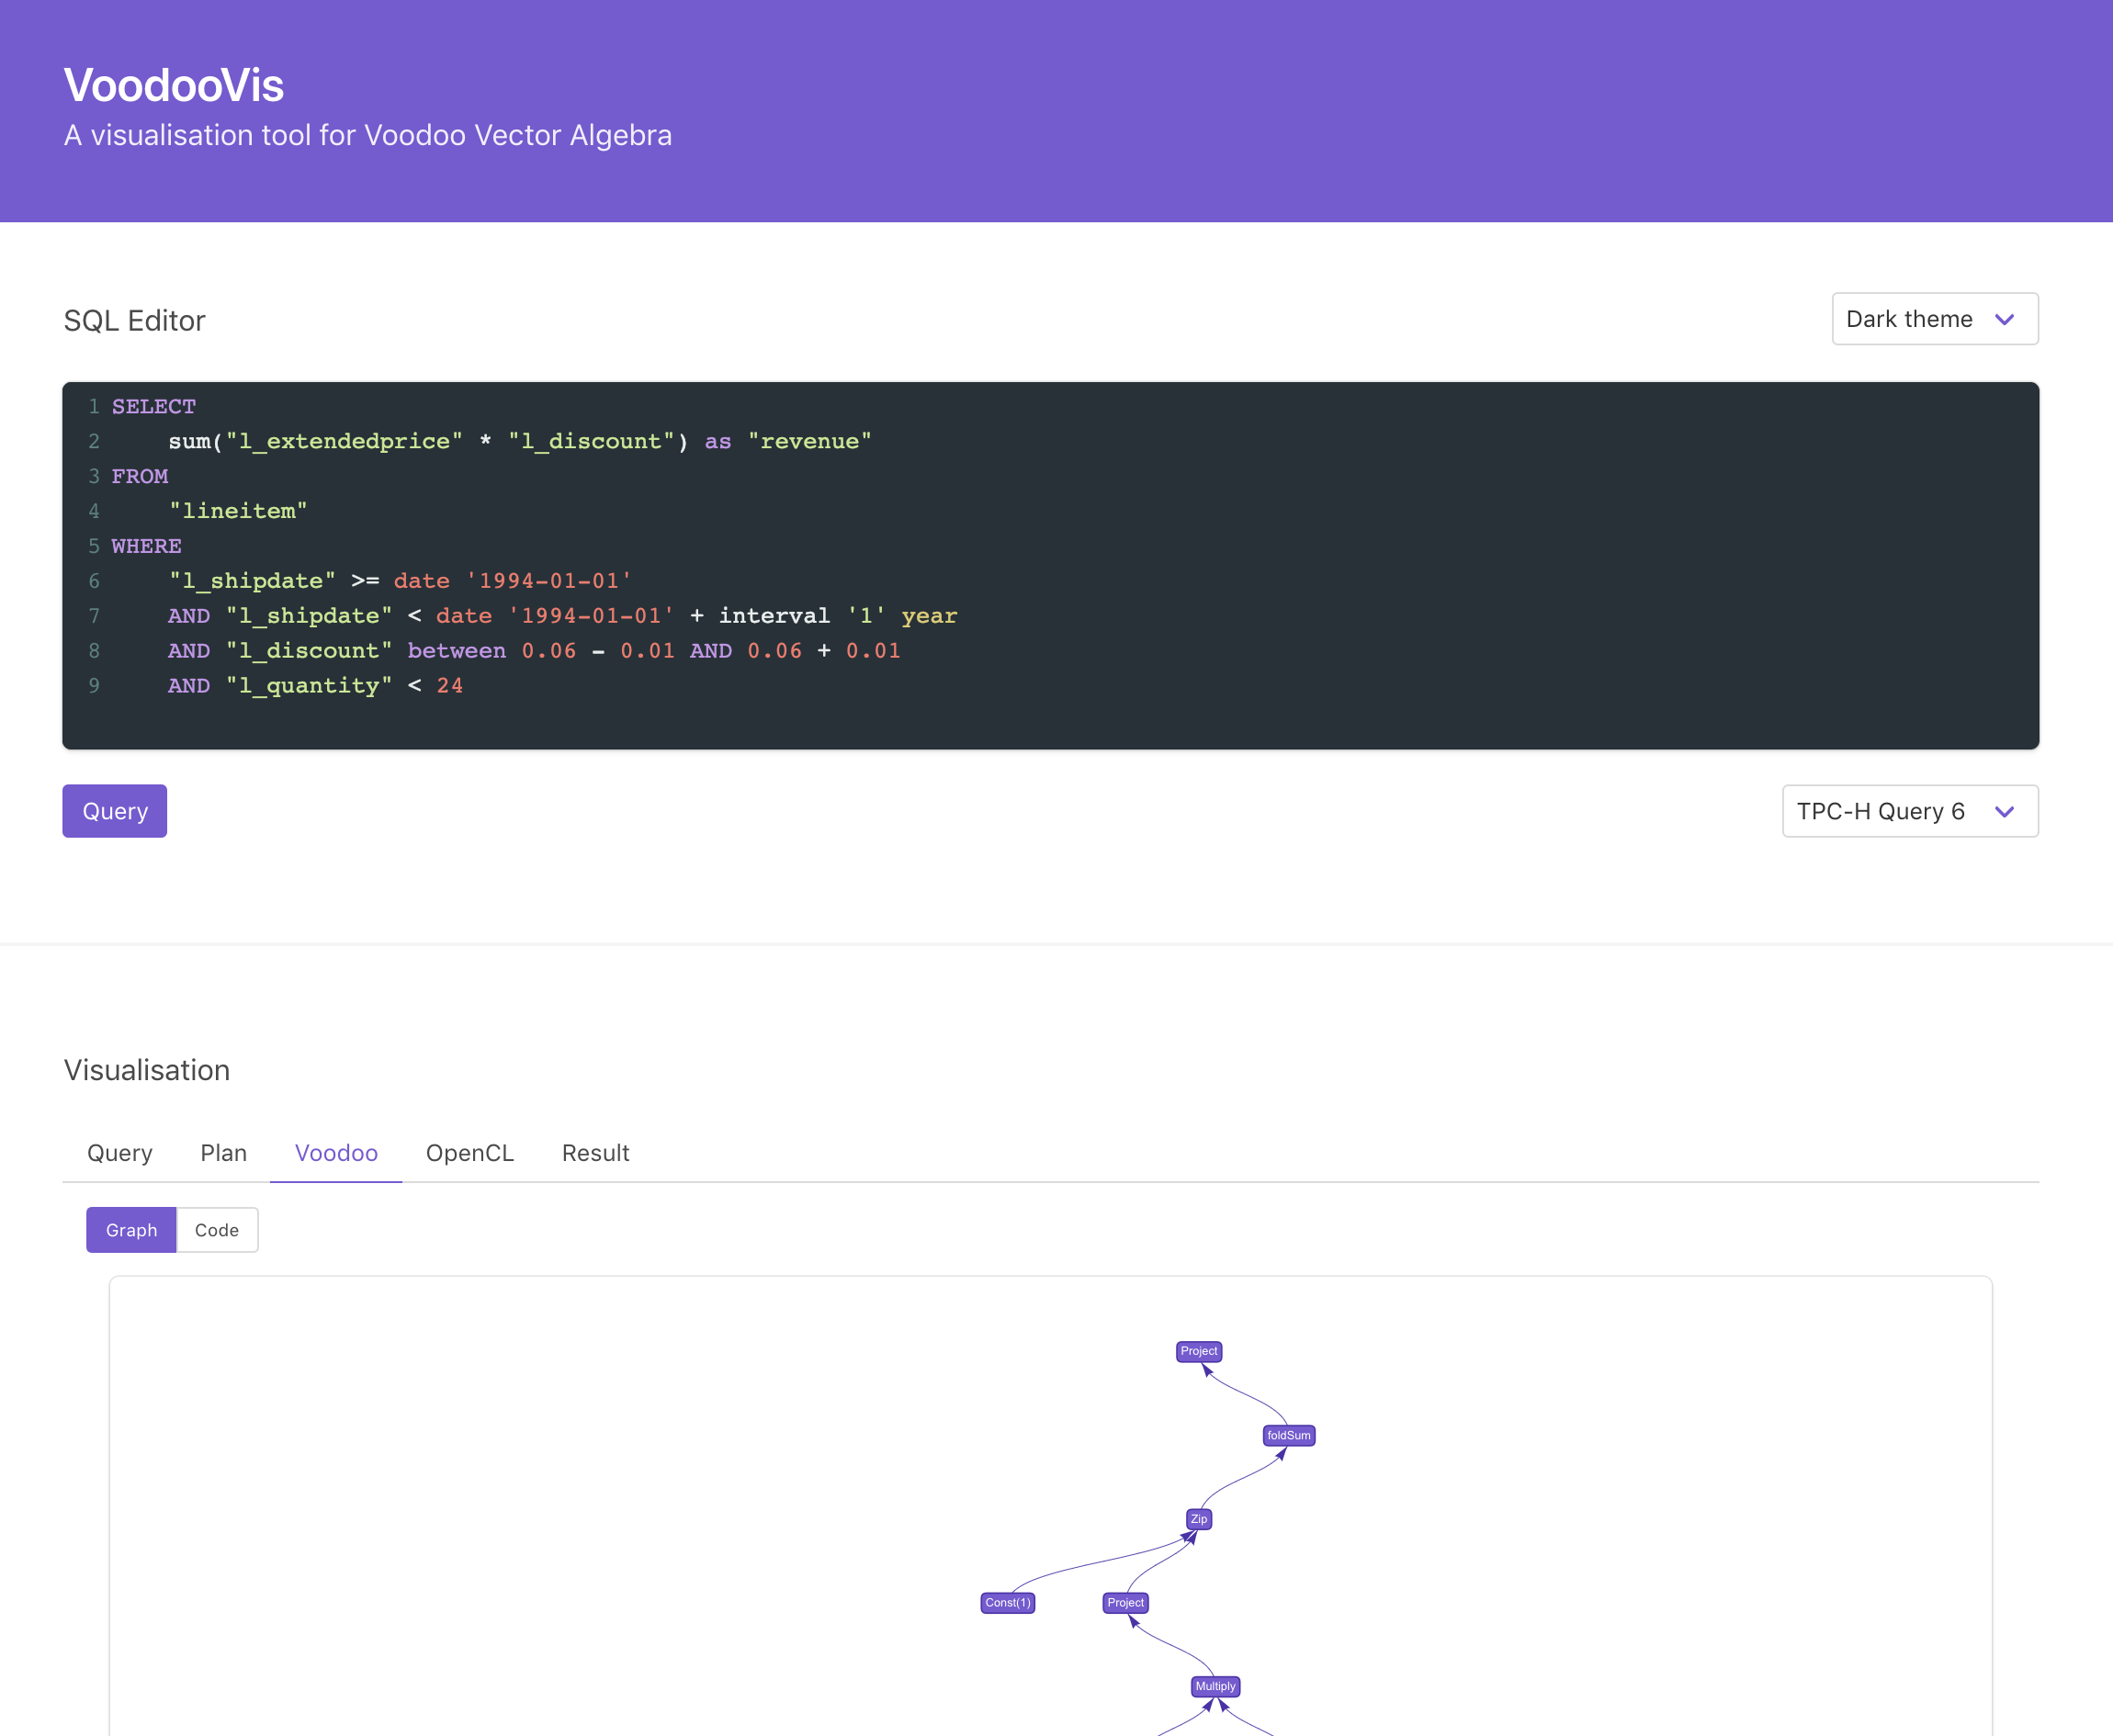
\includegraphics[width=0.95\linewidth]{appendix/q6-screenshot.png}
    \caption{Example of TPC-H query 6 on the visualisation website}
    \label{fig:q6-vis}
\end{figure}
